%!TeX root=../tese.tex
%("dica" para o editor de texto: este arquivo é parte de um documento maior)

% Conteúdo da subseção sobre Bônus
% Este arquivo é importado em 02-implementacao.tex

No contexto do piloto BikeSP, os bônus
representam uma ferramenta complementar de incentivo financeiro aos participantes,
independente das remunerações por quilômetro pedalado. Conforme planejado no desenho
do experimento, os bônus servem a múltiplos propósitos: (i) recompensar a conclusão
do curso gratuito ``Pedale com Segurança'' oferecido pelo Centro de Treinamento e
Educação de Trânsito (CETET) da CET, que treinou centenas de participantes do piloto em técnicas de ciclismo seguro no trânsito urbano; (ii) incentivar o preenchimento dos
questionários qualitativos aplicados em três momentos do piloto, garantindo maior
taxa de resposta e riqueza de dados; (iii) permitir ajustes administrativos e
correções pontuais de pagamento quando necessário; e (iv) viabilizar eventuais
campanhas promocionais temporárias para estimular a participação em momentos
estratégicos do experimento.\footnote{Inserir uma imagem do curso ``Pedale com Segurança'' aqui.}

O painel administrativo oferece três
funcionalidades principais relacionadas a bônus: criação de novos tipos de bônus,
atribuição de bônus a usuários, e visualização e gerenciamento dos bônus
cadastrados. A arquitetura do sistema foi projetada para oferecer flexibilidade e controle sobre os incentivos.

Os administradores podem cadastrar novos tipos de bônus
informando nome único (identificador), valor em reais, descrição textual, período
de validade (datas de início e fim, opcionais), e dois flags de controle: se o
bônus deve ser ativado automaticamente após criação, e se será visível aos
usuários no aplicativo móvel. A distinção entre bônus ativos/inativos e
visíveis/invisíveis oferece grande flexibilidade: bônus inativos não podem ser
concedidos (útil para pausar temporariamente um incentivo), enquanto bônus
invisíveis, mesmo quando concedidos e gerando remuneração, não aparecem na
listagem do aplicativo do usuário (útil para ajustes administrativos discretos ou
correções pontuais). A Figura~\ref{fig:bonus_criar_form} mostra o formulário de criação.

 \begin{figure}[htb]
   \centering
   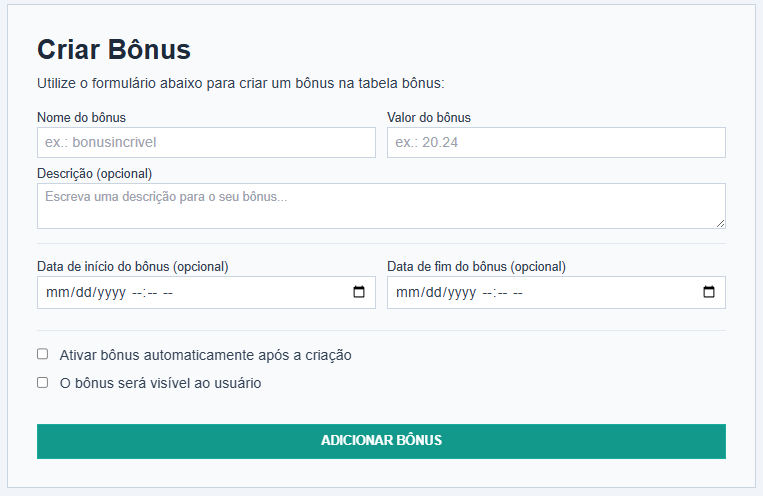
\includegraphics[width=0.95\textwidth]{figuras/criar_bonus.PNG}
   \caption{Formulário de criação de bônus no painel administrativo.}
   \label{fig:bonus_criar_form}
 \end{figure}

Para conceder um bônus a participantes, o
administrador informa os IDs dos usuários (separados por vírgula) e seleciona o
bônus desejado. O sistema valida diversas condições antes de processar a
concessão: o bônus deve estar ativo, não pode ter expirado (data de término não
ultrapassada), todos os usuários devem existir, e cada usuário pode receber cada
bônus apenas uma vez. Ao conceder um bônus com sucesso, o sistema não apenas registra a concessão, mas
também cria automaticamente uma remuneração correspondente ao valor do bônus e a
insere na fila de pagamentos (para posterior transferência aos cartões Bilhete
Único via Loja Virtual SPTrans). Caso algum usuário não atenda aos critérios, o
sistema reporta sucesso parcial, detalhando quantos usuários receberam o bônus e
quais apresentaram erros (por exemplo, ``5 sucessos, 2 erros: Usuário 101 já
possui este bônus; Usuário 203 não existe''). Esta funcionalidade de concessão em
lote reduz significativamente o tempo necessário para operações recorrentes, como
conceder o bônus do curso de segurança para todos os participantes que o
concluíram em determinada semana. A Figura~\ref{fig:bonus_atribuir_form} ilustra esta interface.

 \begin{figure}[htb]
   \centering
   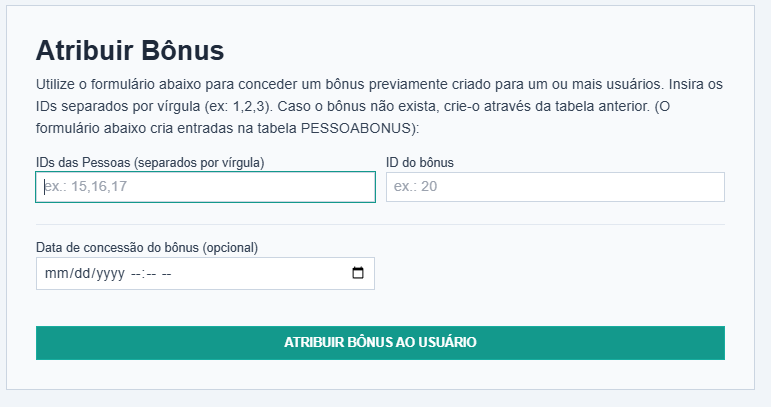
\includegraphics[width=0.95\textwidth]{figuras/atribuir_bonus.PNG}
   \caption{Formulário de atribuição de bônus aos participantes.}
   \label{fig:bonus_atribuir_form}
 \end{figure}

A tela de listagem exibe todos os bônus
cadastrados em formato tabular, apresentando ID, nome, valor, status de ativação,
visibilidade, descrição, período de validade e ações disponíveis. A interface
oferece busca por nome e paginação (5 itens por página). Cada linha da tabela
possui um botão para ativar ou desativar o bônus: bônus ativos exibem
botão vermelho ``Desativar'', enquanto bônus inativos exibem botão verde
``Ativar''. Importante notar que desativar um bônus não remove concessões já
realizadas nem afeta remunerações já geradas; apenas impede novas concessões
daquele tipo de bônus. Para facilitar a identificação dos IDs de usuários ao
atribuir bônus, a aba de bônus também oferece uma consulta integrada à tabela de
usuários, com busca por nome ou ID, ordenação por qualquer coluna e
paginação configurável da mesma forma que a tela de usuários. A Figura~\ref{fig:bonus_listagem_form} mostra a listagem de bônus (dados fictícios para fins ilustrativos).

\begin{figure}[htb]
    \centering
    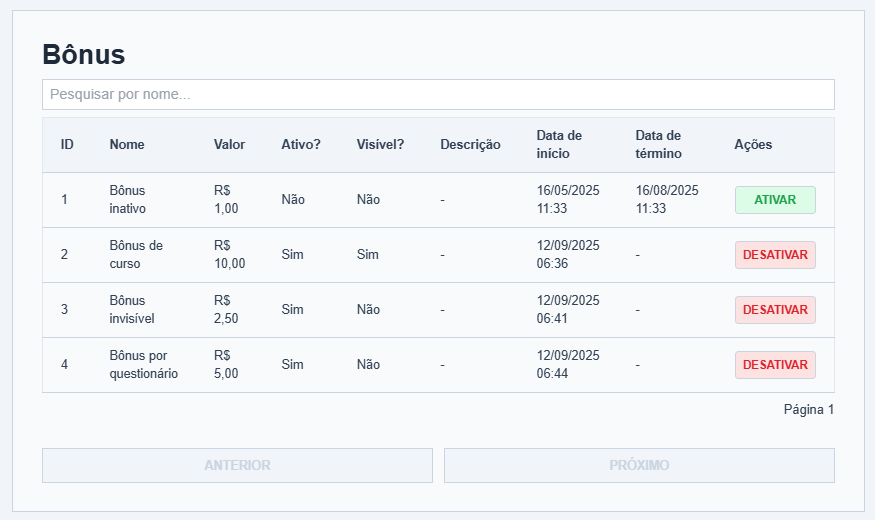
\includegraphics[width=0.95\textwidth]{figuras/bonus_listar.PNG}
    \caption{Listagem de bônus cadastrados com funcionalidades de busca, paginação e ativação/desativação (dados fictícios).}
    \label{fig:bonus_listagem_form}
  \end{figure}
 

O aplicativo Android dos participantes
consome a API \texttt{POST /api/exibeBonus/} para listar os bônus concedidos ao
usuário autenticado. A API retorna apenas bônus marcados como visíveis, garantindo que ajustes administrativos invisíveis não
apareçam para os usuários finais. Esta separação entre visibilidade e concessão
oferece aos gestores do piloto a flexibilidade de realizar correções financeiras
sem necessariamente comunicá-las explicitamente aos participantes.

Durante a execução do piloto, a
funcionalidade de bônus mostrou-se fundamental para diversos cenários operacionais:
concessão em lote do bônus do curso de segurança para centenas de participantes que
o concluíram simultaneamente; distribuição dos bônus dos questionários ao final de
cada período de coleta de dados qualitativos; correções pontuais quando erros de
geolocalização resultaram em viagens rejeitadas indevidamente (criando-se bônus
invisíveis de ajuste); A flexibilidade do sistema permitiu à
equipe operacional responder rapidamente a diferentes necessidades sem requerer
desenvolvimento de novas funcionalidades ou intervenções manuais no banco de dados.



